\documentclass[11pt, a4paper, twocolumn]{article}

% Fonts and math (Elsevier-like Times style)
\usepackage{graphicx} % Required for inserting images
\usepackage{array} % For extra column formatting
\usepackage{amsmath, amssymb, cancel, siunitx, mathtools, physics2, upgreek} % for equation environment
\usepackage{float,geometry,subcaption, longtable}
\geometry{margin=2cm}
\usepackage[skip=10pt]{parskip}
\usepackage{setspace}
\usepackage{hyperref, cleveref}
\usepackage{cite, bookmark}
\usepackage{url}
\usepackage[table,xcdraw]{xcolor}
\usepackage[export]{adjustbox}
\usepackage{listings,pdfpages}
\usepackage{dblfloatfix}

% --- Abstract styling (elsarticle look)
\usepackage{abstract}
\renewcommand{\abstractnamefont}{\normalfont\bfseries}
\renewcommand{\abstracttextfont}{\normalfont}
\renewenvironment{abstract}{%
  \par\noindent\rule{\linewidth}{0.4pt}\par
  \begin{center}\bfseries Abstract\end{center}%
}{%
  \par\rule{\linewidth}{0.4pt}\par
}

% --- Section styling (similar to elsarticle
\usepackage{titlesec}
\titleformat{\section}{\normalfont\large\bfseries}{\thesection.}{0.5em}{}
\titleformat{\subsection}{\normalfont\normalsize\bfseries}{\thesubsection.}{0.5em}{}

% Table of contents styling
\usepackage{tocloft}
\cftsetindents{section}{0em}{2em}
\cftsetindents{subsection}{1em}{2em}
\renewcommand\cfttoctitlefont{\hfill\Large\bfseries}
\renewcommand\cftaftertoctitle{\hfill\mbox{}}
\renewcommand\cftfigfont{\footnotesize}
\renewcommand\cftfigpagefont{\footnotesize}
\renewcommand\cftloftitlefont{\large}

\graphicspath{ {./images/} }

\definecolor{blurple}{HTML}{5865F2}
\definecolor{backcolour}{HTML}{272823}

\hypersetup{
    colorlinks=true,
    linkcolor=black,
    urlcolor=black,
    citecolor=blurple,
}

\urlstyle{same}

\DeclareMathOperator{\sinc}{sinc}

\renewcommand{\arraystretch}{1.4}

% Python code export
\lstset{
    language=Python,
    basicstyle=\ttfamily\scriptsize,
    keywordstyle=\color{magenta},       
    commentstyle=\color{gray},        
    stringstyle=\color{teal},  
    showstringspaces=false,
    frame=single,
    breaklines=true,
    numbers=left,
    numberstyle=\tiny\color{gray}
}

\setcounter{secnumdepth}{5}
\setcounter{tocdepth}{5}

\hbadness=99999

%%%%%%%%%%%%%%%%%%%%%%%%%%%%%%%%%%%

\title{%


\includegraphics[width=0.2\linewidth]{ucd_brandmark_black.jpg} \vspace{0.5cm}\\

{\Large\bfseries UCD School of Physics}\vspace{1.5cm}\\

{\large PHYC30170 Physics Astronomy and Space Lab I}\\
{\bfseries Compton Scattering}

}
\author{Joana C.C. Adao \\ \small Student No.: 23311051}
\date{\today}

\begin{document}

% Title page - single column
\onecolumn
\maketitle

% Abstract - single column
\pagenumbering{roman}
\setcounter{page}{1}
\begin{abstract}

This experiment sought to investigate the fundamental aspects of the Compton scattering phenomenon using a Cs-137 gamma-ray source (0.6617 Mev) and a NaI(Tl) scintillation detector. The energy and differential cross-section of the scattered photons were measured at angular range of 20°-90° and compared to the theoretical predictions to validate the relativistic kinematics and the Klein-Nishina formula. A linear regression of $1/E_{\gamma'}$ against $(1-\cos\theta)$ yielded an experimental slope of \textbf{2.030 ± 0.012} and y-intercept of \textbf{1.58 ± 0.007}, with percentage errors of \textbf{3.77\%} and \textbf{4.68\%} respectively relative to theoretical calculations of \textbf{1.956} and \textbf{1.51}. While the plot of the differential cross-section showed a similar trend to the Klein-Nishina theoretical trend, the experimental values remained systematically lower than expected, suggesting systematic errors in the measurements.

\end{abstract}

\newpage

% Table of Contents - single column
\tableofcontents

\newpage

%%%%%%%%%%%%%%%%%%%%%%%%%%%%%%%%%%%

% Start main content in two columns
\twocolumn
\pagenumbering{arabic}
\setcounter{page}{1}

\section{Introduction} \label{sec:1}

Compton scattering describes the inelastic scattering of a photon from a nearly free electron, resulting in a change in the photon's energy, wavelength, and momentum, providing valuable information about how light interacts with matter. 

\begin{figure}[H]
  \centering
  
\includegraphics[width=.9\linewidth]{compton.png}
  \caption{Geometry of Compton Scattering. \cite{venugopal}}
  \label{fig:1}
  \vspace{-1.2ex}
\end{figure}

The incident (gamma-ray) photon with energy $E_{\gamma}=h\nu$ collides with an electron of energy $E_{\gamma'}=h\nu'$ assumed to be initially at rest, and the scattered photon deflects at an angle $\theta$ with respect to the original direction, illustrated in \autoref{fig:1}. \cite{knoll2010radiation,cryst11050525,UCD_PHYC30090_Part3,UCD_comptonlab}

\subsection{Kinematics}

The behaviour of the scattered photon follows the energy and momentum conservation laws, which can be expressed as \cite{UCD_comptonlab}:

\vspace{-2ex}
\begin{gather}
  E_{\gamma} = E_{\gamma'} + E_e \\[2ex]
  \text{(x-dir.)}\quad \frac{h\nu}{c} = \frac{h\nu'}{c}\cos\theta + mv\cos\phi \\
  \text{(y-dir.)}\quad\; 0 = \frac{h\nu'}{c}\sin\theta - mv\sin\phi
\end{gather}

With the use of these conservations of energy and momentum, the energy of the scattered photon can be derived to show \cite{knoll2010radiation,UCD_PHYC30090_Part3,UCD_comptonlab,cryst11050525,PRATT2010124}:

\begin{equation} \label{eq:1}
  E_{\gamma'} = \frac{E_{\gamma}}{1+\frac{E_{\gamma}}{m_0c^2}(1-\cos\theta)}
\end{equation}

where $m_0c^2$ is the energy of the rest electron (0.511 MeV). This can then be expressed in terms of wavelength shift as \cite{UCD_PHYC30090_Part3,rybicki2024radiative}:

\begin{equation}
  \Delta\lambda = \lambda' - \lambda = \frac{h}{m_0c}(1-\cos\theta)
\end{equation}

where $h/m_0c$ is the Compton wavelength of the electron (\qty{2.426e-10}{cm}). The maximum wavelength shift thus occurs at $\theta=180^{\circ} \; \text{or}\; \pi$ radians, and the minimum shift occurs through forward scattering at $\theta=0 \;(^{\circ}\;\text{or radians})$. \cite{UCD_PHYC30090_Part3}

\subsection{Differential Cross-Section}

The probability of scattering at a given angle is described by the electronic differential cross-section, defined using relativistic quantum mechanics, and given by the Klein-Nishina formula \cite{UCD_PHYC30090_Part3,UCD_comptonlab,knoll2010radiation,rybicki2024radiative,PRATT2010124,cryst11050525}:

\begin{multline} \label{eq:3}
  \frac{d\sigma}{d\Omega} = \frac{r_0^2}{2} \left\{ \frac{1+\cos^2\theta}{[1+\alpha(1-\cos\theta)]^2} \right\} \times \\
  \left\{ 1 + \frac{\alpha^2(1-\cos\theta)^2}{(1+\cos^2\theta)(1+\alpha[1-\cos\theta])} \right\}
\end{multline}

where $d\sigma/d\Omega$ is the differential cross-section, $r_0$ is the classical electron radius (\qty{2.8e-13}{cm}), $\alpha = E_{\gamma}/m_0c^2$. As energy increases, the scattering cross-section decreases, indicating that high-energy photons are less likely to scatter than low-energy photons. For low-energy photons ($\alpha \ll 1$) the formula reduces to the non-relativistic Thomson scattering cross-section, which is independent of energy \cite{UCD_PHYC30090_Part3,rybicki2024radiative,cryst11050525,PRATT2010124}:

\begin{equation}
  \frac{d\sigma}{d\Omega} = \frac{r_0^2}{2}(1+\cos^2\theta)
\end{equation}

Additionally, the probability of scattering depends on the number of electrons available in the target material, and thus increases linearly with the atomic number $Z$ as ${}_a\sigma_c = Z\, {}_e\sigma_c$, where ${}_a\sigma_c$ is the \textit{atomic} Compton scattering cross-section and ${}_e\sigma_c$ is the \textit{electronic} Compton scattering cross-section. \cite{UCD_PHYC30090_Part3,knoll2010radiation}

\section{Methodology} \label{sec:3}

The experimental setup for Compton scattering, illustrated in \autoref{fig:2}, used a high activity Cs-137 gamma-ray source (1) housed within lead bricks to minimise background radiation, and a 2"x2" NaI(Tl) scintillation detector (4) was mounted on a pivoting arm to measure the scattered photons at various angles between 20° and 90°. A collimator (3) was used to narrow the gamma-ray beam for detection, and a target of the scattering sample (2) was placed at the pivot point. 

\begin{figure}[ht]
  \centering
  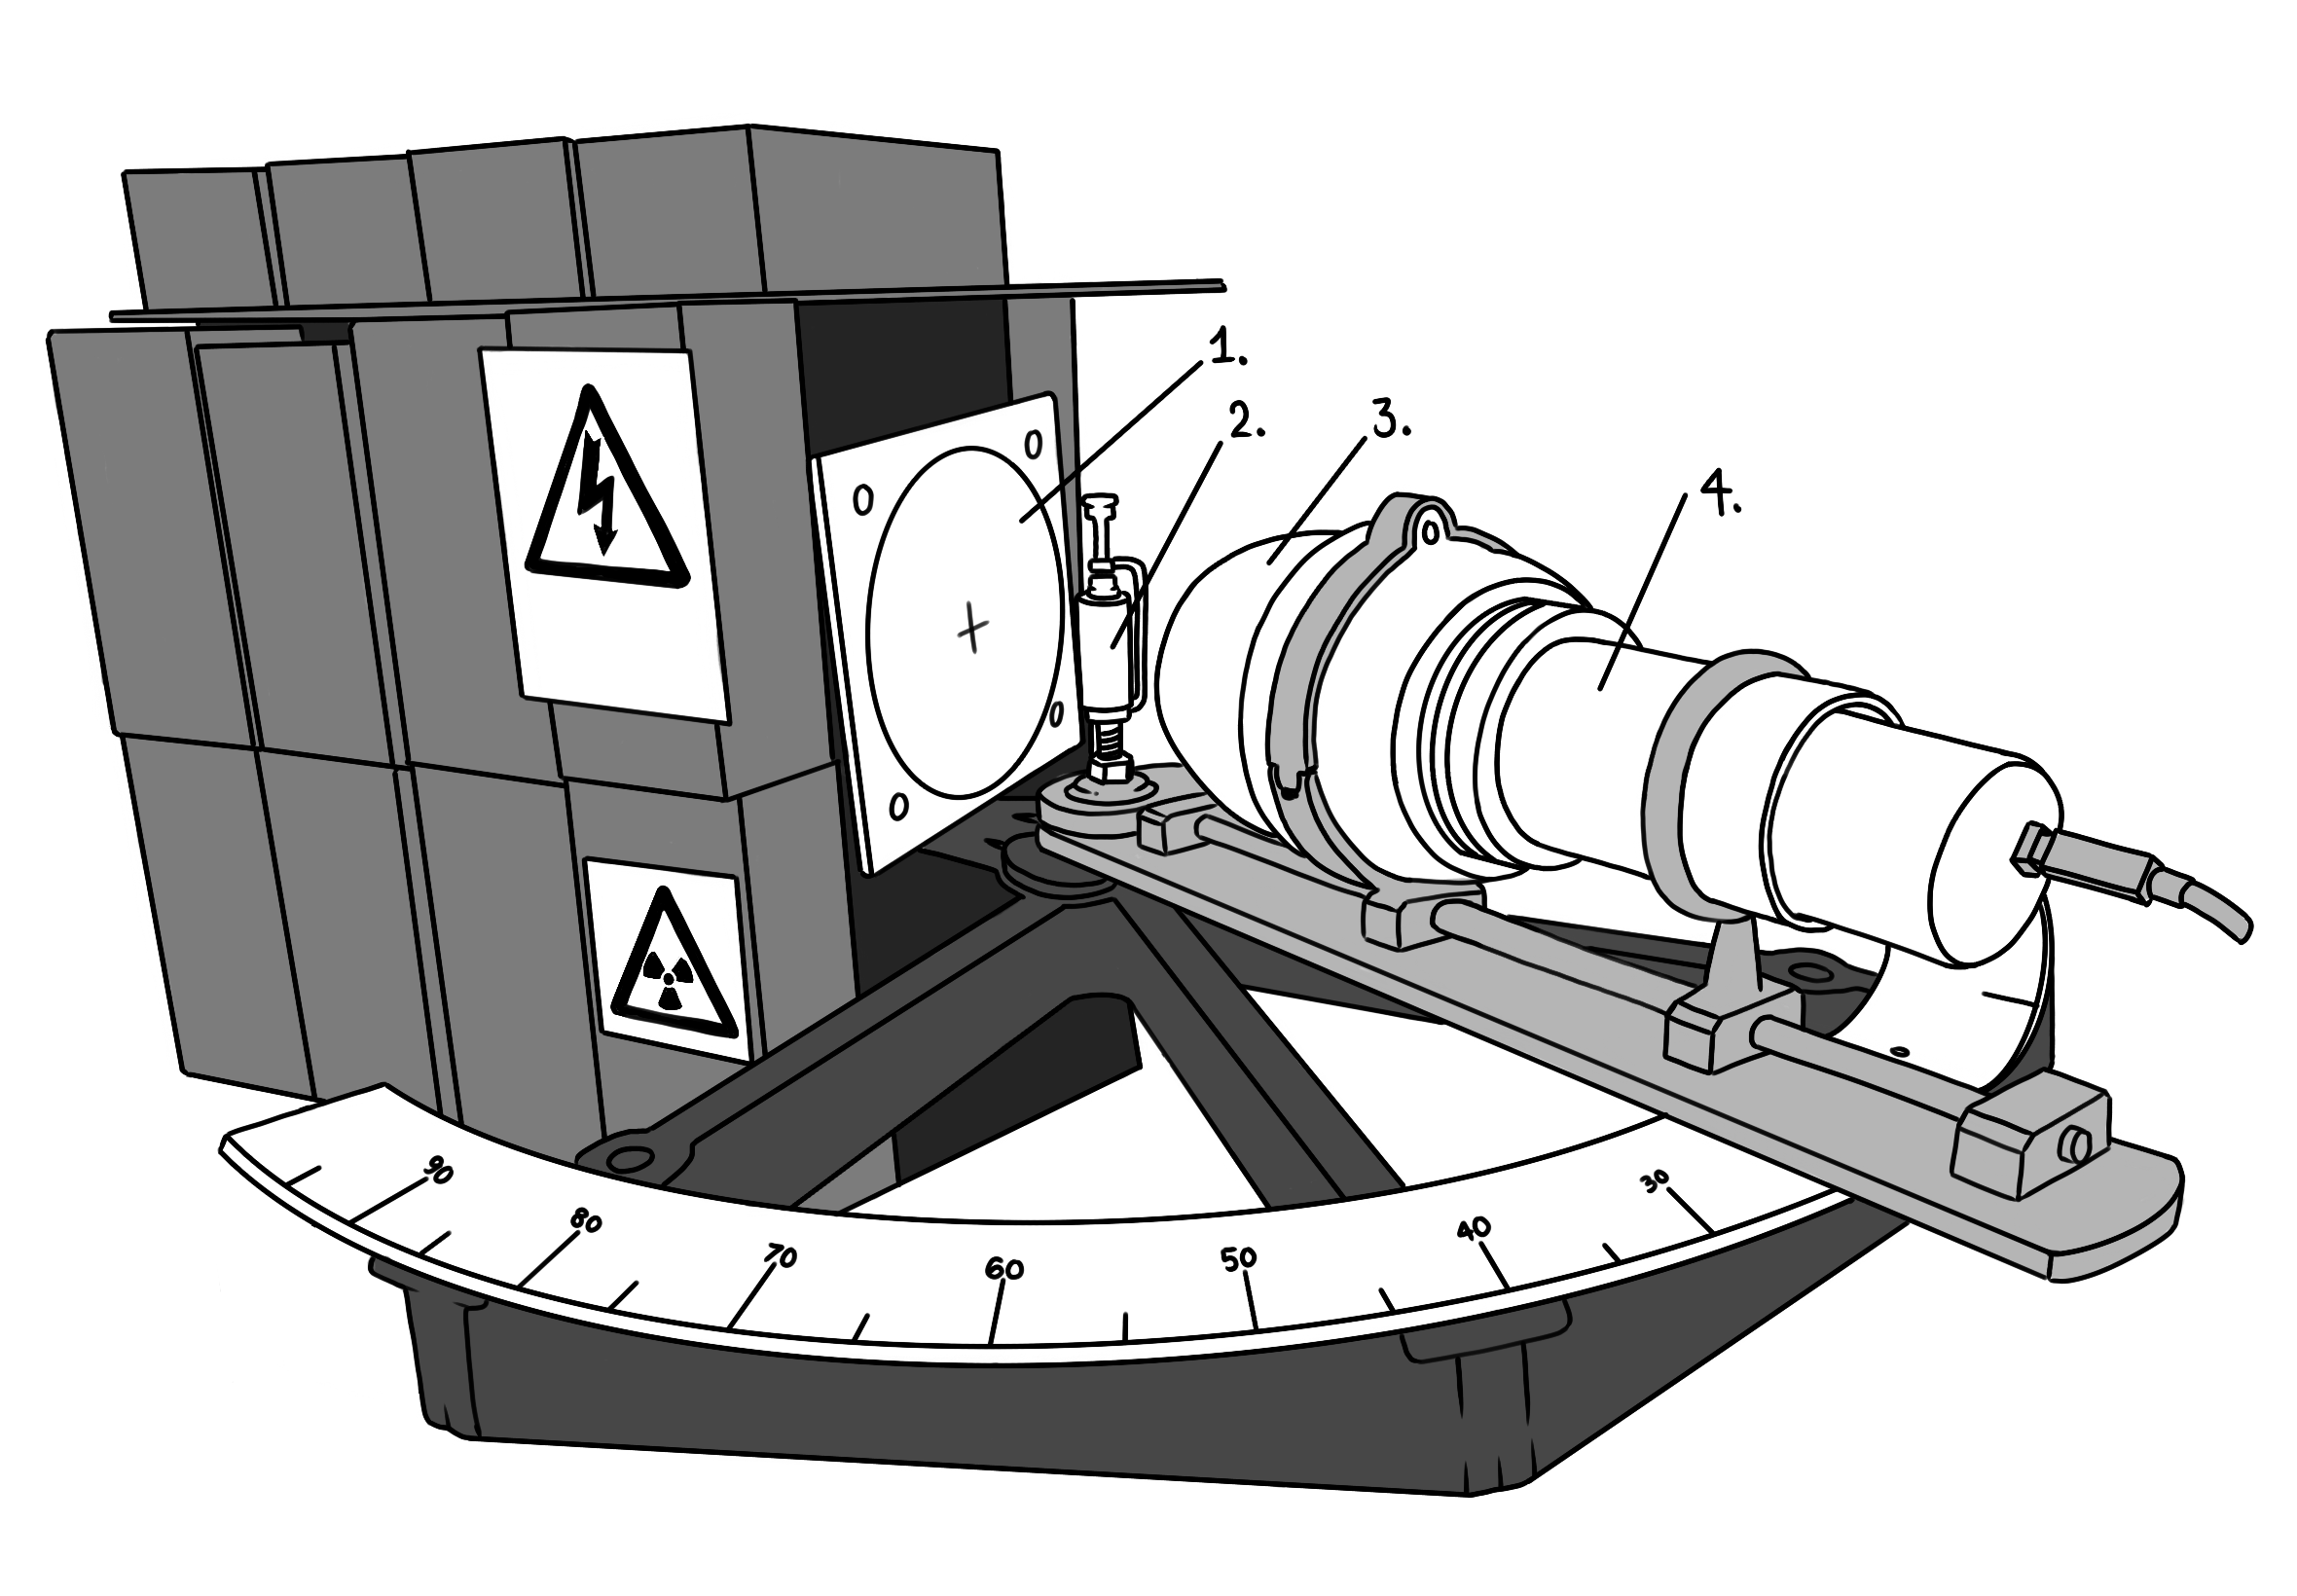
\includegraphics[width=\linewidth]{comptonexp.PNG}
  \caption{Illustration of the experimental setup for Compton scattering with a 2"x2" NaI(Tl) scintillation detector; \textit{1. Cs-137 source, 2. Target, 3. Collimator, 4. Photomultiplier tube (PMT), amplifier, and scintillation detector}}
  \label{fig:2}
  \vspace{-1ex}
\end{figure}

The incoming scattered gamma-ray photons were amplified and measured at the PMT once they had interacted with the scintillation detector, and the electrical signals were processed in the \textit{Maestro-32} software to obtain the energy spectra and photopeaks. 

\subsection{Calibration of the Software}

To calibrate the software, a sample of Am-241 and Cs-137 were used with their known photopeak energies of 59.5 keV and 662 keV, respectively, and comparing to the channel numbers of the measured photopeaks. The software created its own calibration curve within it, which was used for all further measurements. 

Tweezers were used to handle the portable samples and the samples were placed directly in front of the detector and measured until a peak was seen to form. When not in use, all radioactive samples were stored in a locker in accordance with safety protocols and regulations.

\subsection{Measurement Acquisition}

To begin measurements, the source aperture was opened, and the detector positioned at the desired angle. The spectrum was recorded until a net count of at minimum 10,000 counts were obtained under the photopeak using the software. Measurements were taken at angle increments of 5°, and the respective net counts, count uncertainties (given by software), peak energies (in keV), and time taken for each measurement were recorded in a table. 

Plots for the energy of the scattered photon and the differential cross-section, both as a function of the scattering angle, were plotted and compared graphically to theoretical predictions from \autoref{eq:1} and \autoref{eq:3} respectively.

\section{Results} \label{sec:4}

When calibrating the software, the obtained channels for the Am-241 and Cs-137 photopeaks were \textbf{89} and \textbf{850} respectively, and inputted into a window within the software to implicitly create a calibration curve. Time taken, scattering angle, and net counts and uncertainties were unnecessary for the calibration and thus not recorded.

\subsection{Kinematics}

The scattering angles were converted into radians and the energies into MeV for comparison to the theoretical predictions. A plot of $1/E_{\gamma'}$ against $(1-\cos\theta)$ was made and fitted with a linear regression, shown in \autoref{fig:3}.

\begin{figure} [H]
  \centering
  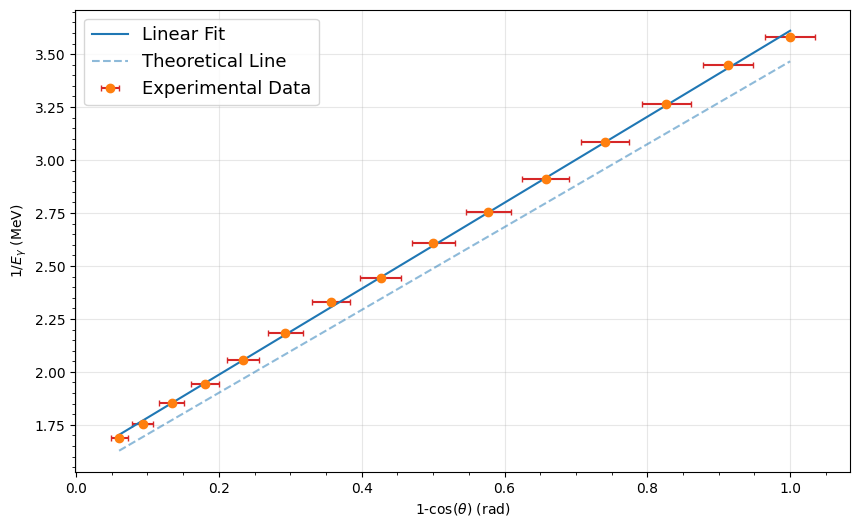
\includegraphics[width=.95\linewidth]{comptonEplot.png}
  \caption{Plot of $1/E_{\gamma'}$ against $(1-\cos\theta)$ in radians with linear regression fit.}
  \label{fig:3}
  \vspace{-1.2ex}
\end{figure}

A value for the slope and y-intercept were obtained from the linear fit line, \textbf{2.030 ± 0.012} and \textbf{1.58 ± 0.007} respectively. Comparing to the theoretical predictions of \textbf{1.956} for the slope and \textbf{1.51} for the y-intercept, the experimental percentage errors were calculated to be \textbf{3.77\%} and \textbf{4.68\%} respectively. 

The error on the scattering angle was estimated to be ±2° due to obstruction of the angle markings by the pivot arm and difficulty in moving the detector in small, precise increments. The error on the energy was not given by the software and thus not included in the error analysis.

\subsection{Differential Cross-Section}

From the values obtained for the net counts and time taken for each measurement, a series of calculations were performed to obtain the experimental values for the differential cross-section, which were plotted against the scattering angle and compared to the Klein-Nishina theoretical prediction, shown in \autoref{fig:4}.

\begin{figure}[H]
  \centering
  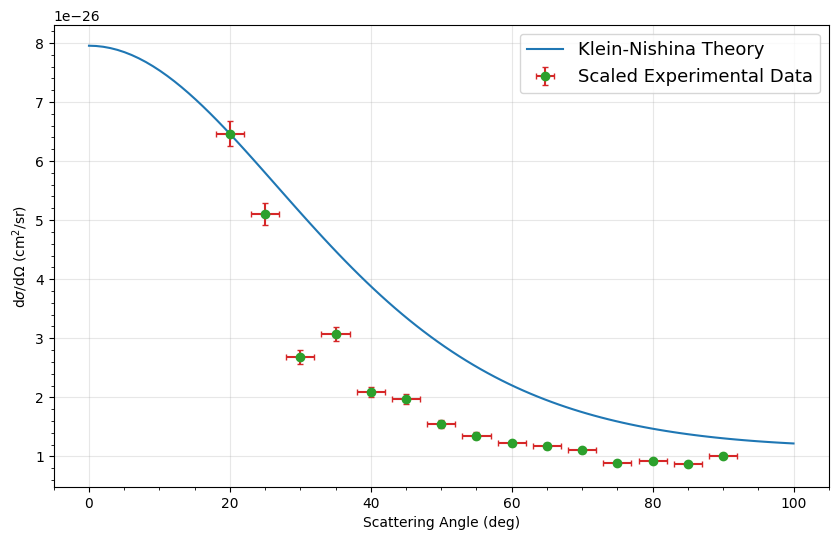
\includegraphics[width=.95\linewidth]{comptonCSplot.png}
  \caption{Plot of $d\sigma/d\Omega$ against scattering angle $\theta$ in degrees, with theoretical prediction from the Klein-Nishina formula.}
  \label{fig:4}
  \vspace{-1.2ex}
\end{figure}

The solid angle $\Delta\Omega$ of the detector was calculated using $\Delta\Omega = A/R_2^2$, with $A$ as the area of the detector (\qty{5}{cm}) and $R_2$ as the distance from the detector to the target (\qty{26}{cm}). The number of electrons in the target was calculated using $N_e = Z_{\text{Al}}N_aM/A_{\text{Al}}$, where $Z_{\text{Al}}$ is the atomic number of aluminium (13), $N_a$ is Avogadro's number, $M$ is the mass of the target (\qty{79.3}{g}), and $A_{\text{Al}}$ is the molar mass of aluminium (\qty{26.9815}{g/mol}). The intrinsic efficiency of the detector was calculated using $E_{\text{eff}}=0.1522(E)^{-1.1325}$, with $E$ as the energy of the scattered photon (MeV). The count rate $R$ was calculated using $R=N/t$, where $N$ is the net counts and $t$ is the time taken per measurement. The cross-section was then calculated using $(\partial\sigma/\partial\Omega) = R/N\Delta\Omega E_{\text{eff}}$.

The experimental values were scaled to the Klein-Nishina prediction at $\theta=20^{\circ}$. The shape of the experimental plot follows the same trend as the theoretical prediction but with lower values, which may indicate to systematic errors in the measurements.

\section{Analysis and Discussion} \label{sec:5}

The linear relationship observed in \autoref{fig:3} is consistent with the theoretical prediction from \autoref{eq:1} using the Cs-137 gamma-ray source (0.6617 MeV). The results obtained for the slope of $\mathbf{2.030 \pm 0.012}$ and y-intercept of $\mathbf{1.58 \pm 0.007}$ are relatively close to the theoretical predictions of \textbf{1.956} and \textbf{1.51} respectively, with percentage errors of \textbf{3.77\%} and \textbf{4.68\%} respectively.

The likely sources of error in the measurements include the estimated error on the scattering angle of ±2° due to mechanical limitations of the pivot arm in moving it in small increments and the obstruction of the angle markings. Errors when calibrating the software may have also contributed to the errors observed, which could have arisen from misplacing the samples in front of the detector or not measuring for long enough to obtain a clear photopeak. The experimental fit is observed to diverge more from the theoretical prediction at higher scattering angles, which may have been mitigated by taking more counts at all angles to reduce the statistical error.

The plot of the differential cross-section in \autoref{fig:4} shows a similar trend to the theoretical prediction obtained from the Klein-Nishina formula by following the expected behaviour of the probability of scattering decreasing with the increasing scattering angle. However, the experimental values were consistently lower than the theoretical line, even after scaling the data to the Klein-Nishina prediction at $\theta=20^{\circ}$, which suggests presence of systematic errors in the measurements rather than random errors or fluctuations.

The likely sources of error could be partly due to the Cs-137 source, which was obtained in the 1970s and thus may have had a reduced activity due to decay, thus necessitating longer measurement times to obtain more counts to reduce the statistical error, and could have influenced signal-to-noise ratio in the software and the accuracy of the net counts obtained. Additionally, the NaI(Tl) scintillation device efficiency is influenced by age and temperature most notably, and thus the accuracy of the general efficiency formula used may have led to the underestimation of the experimental values. Another source of error could be the estimation of the solid angle of the detector, which generally assumer a point source and flat detector surface, for which the target may have caused angular smearing by measuring over a range of angles rather than a single angle.

Despite these discrepancies, the results obtained for both the kinematics and the differential cross-section show the expected respective trends and are relatively close to the theoretical predictions, even if not in perfect agreement.

\section{Conclusion}

The results of this experiment provide evidence for the Compton scattering phenomenon and strong support for the theoretical predictions of the energy of the scattered gamma-ray photon and the differential cross-section as a function of the scattering angle. The linear relationship observed in the plot of $1/E_{\gamma'}$ against $(1-\cos\theta)$ in \autoref{fig:3} is consistent with the expected behaviour from the Compton scattering formula. The small percentage errors obtained for the slope and y-intercept values demonstrate that the experimental setup was capable of accuracy despite mechanical limitations, particularly in the measurement and alignment of the scattering angles.

The plot of the differential cross-section in \autoref{fig:4} also shows a similar trend as to expectations with the theoretical prediction from the Klein-Nishina formula, though the underestimation of the experimental values showed the difference between the idealised theoretical model and the realistic experimental setup with its various sources of systematic errors.

Despite the errors present in the measurements, the results obtained provide strong evidence and support for the theory that underlines the Compton scattering phenomenon, and the experiment was successful in demonstrating the expected behaviours and providing understading on quantum electrodynamics and the interaction of light with matter.

%%%%%%%%%%%%%%%%%%%%

% References - switch to single column
\onecolumn

\bibliographystyle{IEEEtran}
\bibliography{PHYC30170References} \label{sec:ref}

\newpage

% Appendix - single column
\section*{Appendix} \label{sec:A}
\addcontentsline{toc}{section}{Appendix}

\subsection*{Tables}
\addcontentsline{toc}{subsection}{Tables}

\begin{table}[H]
\centering
\caption{Table of the raw data obtained for the experiment.}
\label{tab:1}
\begin{tabular}{|c|c|c|c|c|}
\hline
\rowcolor[HTML]{EFEFEF} 
Angle (°) & NET count & Count Unc. & Energy (keV) & Live Time (s) \\ \hline
20        & 10852     & 358        & 591.67       & 123.48        \\ \hline
25        & 11112     & 399        & 569.62       & 153.36        \\ \hline
30        & 11156     & 516        & 539.86       & 275.78        \\ \hline
35        & 12553     & 478        & 514.52       & 256.28        \\ \hline
40        & 14329     & 585        & 485.86       & 401.84        \\ \hline
45        & 10583     & 465        & 457.75       & 295.86        \\ \hline
50        & 11493     & 501        & 429.49       & 379.7         \\ \hline
55        & 10800     & 479        & 409.15       & 386.8         \\ \hline
60        & 15131     & 537        & 383.57       & 557.98        \\ \hline
65        & 10310     & 421        & 363.01       & 370.54        \\ \hline
70        & 10420     & 389        & 343.42       & 374.12        \\ \hline
75        & 10540     & 414        & 324.33       & 445.22        \\ \hline
80        & 11269     & 388        & 306.35       & 424.02        \\ \hline
85        & 10068     & 352        & 289.84       & 377.9         \\ \hline
90        & 10104     & 305        & 279.4        & 317.9         \\ \hline
\end{tabular}
\end{table}

\addcontentsline{toc}{subsection}{Code}


\includepdf[pages=1-4]{compton.pdf}

\end{document}